\chapter{Conclusão}
\label{chap:conclusao}

\lipsum[2]

Ola \cite{lamport1986latex}
\cite{Maia2011}

\begin{table}[htb]
	\IBGEtab{%
		\caption{\label{tabela-ibge} Um Exemplo de tabela alinhada que pode ser longa ou curta,
			conforme padrão IBGE.}%		
	}{%
	\begin{tabular}{ccc}
		\toprule
		Nome & Nascimento & Documento \\
		\midrule \midrule
		Maria da Silva & 11/11/1111 & 111.111.111-11 \\
			Maria da Silva & 11/11/1111 & 111.111.111-11 \\
				Maria da Silva & 11/11/1111 & 111.111.111-11 \\
		\bottomrule
	\end{tabular}%
}{%
\fonte{Produzido pelos autores}%
\nota{Esta éuma nota, que diz que os dados são baseados na
	regressão linear.}%
\nota[Anotações]{Uma anotação adicional, seguida de várias outras.}%
}
\end{table}

\cite{Huetal2000}

\section{Exemplo de Algoritmos}
\lipsum[2]

\begin{algorithm}[h!]
	\Entrada{o proprio texto}
	\Saida{como escrever algoritmos com \LaTeX2e }
	\Inicio{
		inicializa\c{c}\~ao\;
		\Repita{fim do texto}{
			leia o atual\;
			\Se{entendeu}{
				vá para o próximo\;
				próximo se torna o atual\;}
			\Senao{volte ao início da seção\;}
		}
	}
	\caption{Como escrever algoritmos no \LaTeX2e}
\end{algorithm}

\lipsum[2]
%\begin{algorithm}[H]
%	\Entrada{o proprio texto}
%	\Saida{como escrever algoritmos com \LaTeX2e }
%	\Inicio{
%		inicializa\c{c}\~ao\;
%		\Repita{fim do texto}{
%			leia o atual\;
%			\Se{entendeu}{
%				vá para o próximo\;
%				próximo se torna o atual\;}
%			\Senao{volte ao início da seção\;}
%		}
%	}
%	\caption{Exemplo de Algoritmo Versao 02}
%\end{algorithm}

%\begin{algorithm}
%	\begin{algorithmic}
%	\Entrada{o proprio texto}
%	\Saida{como escrever algoritmos com \LaTeX2e }	
%	\end{algorithmic}
%\end{algorithm}

\begin{table}[h!]	
	\centering
	\Caption{\label{tab:internal}Internal exon scores}	
	\IBGEtab{}{
    	\begin{tabular}{cll}
    		\toprule
    		Ranking & Exon Coverage & Splice Site Support\\
    		\midrule \midrule
    		E1 & Complete coverage by a single transcript & Both splice sites\\
    		E2 & Complete coverage by more than a single transcript & Both splice sites\\
    		E3 & Partial coverage & Both splice sites\\
    		E4 & Partial coverage & One splice site\\
    		E5 & Complete or partial coverage & No splice sites\\
    		E6 & No coverage & No splice sites\\
    		\bottomrule
    	\end{tabular}
    }{
    	\Fonte{os autores}
    }
\end{table}

\lipsum[2] 

Referenciando a \autoref{tab:internal-44}

\begin{table}[h!]	
	\centering
	\Caption{\label{tab:internal-44}Internal exon scores}
	
	\IBGEtab{}{
    	\begin{tabular}{cll}
    		\toprule
    		Ranking & Exon Coverage & Splice Site Support\\
    		\midrule \midrule
    		E1 & Complete coverage by a single transcript & Both splice sites\\
    		E2 & Complete coverage by more than a single transcript & Both splice sites\\
    		E3 & Partial coverage & Both splice sites\\
    		E4 & Partial coverage & One splice site\\
    		E5 & Complete or partial coverage & No splice sites\\
    		E6 & No coverage & No splice sites\\
    		\bottomrule
    	\end{tabular}
    }{
    	\Fonte{os autores}
    }
\end{table}

\section{Figuras}

\index{figuras}Figuras podem ser criadas diretamente em LaTeX,
como o exemplo da \ref{fig-grafico-1}.

	\begin{figure}[h!]
		\centering
		\Caption{\label{fig-grafico-1}Produção anual das dissertações de mestrado e teses de doutorado entre os anos de 1990 e 2008}		
		\IBGEtab{}{
			\fbox{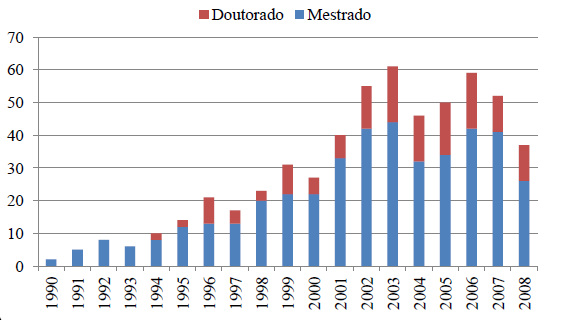
\includegraphics{figuras/figura-3}}
		}{
		\Fonte{os autores}
	}
	\end{figure}

Ou então figuras podem ser incorporadas de arquivos externos, como é o caso da \autoref{fig-grafico-1}. Se a figura que ser incluída se tratar de um diagrama, um gráfico ou uma ilustração que você mesmo produza, priorize o uso de imagens vetoriais no formato PDF. Com isso, o tamanho do arquivo final do trabalho será menor, e as imagens terão uma apresentação melhor, principalmente quando impressas, uma vez que imagens vetorias são perfeitamente escaláveis para qualquer dimensão. Nesse caso, se for utilizar o Microsoft Excel para produzir gráficos, ou o Microsoft Word para produzir ilustrações, exporte-os como PDF e os incorpore ao documento conforme o exemplo abaixo. No entanto, para manter a coerência no uso de software livre (já que você está usando LaTeX e abnTeX),  teste a ferramenta InkScape\index{InkScape}. ao CorelDraw\index{CorelDraw} ou ao Adobe Illustrator\index{Adobe! Illustrator}.  De todo modo, caso não seja possível  utilizar arquivos de imagens como PDF, utilize qualquer outro formato, como JPEG, GIF, BMP, etc.  Nesse caso, você pode tentar aprimorar as imagens incorporadas com o software livre \index{Gimp}Gimp. Ele é uma alternativa livre ao Adobe Photoshop\index{Adobe! Photoshop}.